\documentclass[12pt]{article}
  
\usepackage[margin=1in]{geometry} 
\usepackage{amsmath,amsthm,amssymb,bm,mathtools,scrextend}
\usepackage{fancyhdr}
\pagestyle{fancy}
\usepackage{hyperref}

\usepackage{graphicx}
\usepackage[most]{tcolorbox}
\usepackage{algpseudocode}
\usepackage{algorithm}
\usepackage{listings}

\newcommand{\expect}[1]{\mathbb{E}\left[#1\right]}
\newcommand{\av}{\mathbf{a}}
\newcommand{\rv}{\mathbf{r}}
\newcommand{\cv}{\mathbf{cv}}
\newcommand{\C}{\mathbf{C}}
\newcommand{\n}{\mathbf{n}}
\newcommand{\q}{\mathbf{q}}
\newcommand{\x}{\mathbf{x}}
\newcommand{\y}{\mathbf{y}}
\newcommand{\z}{\mathbf{z}}
\newcommand{\0}{\mathbf{0}}
\newcommand{\1}{\mathbf{1}}
\newcommand{\I}{\mathbf{I}}
\newcommand{\X}{\mathbf{X}}
\newcommand{\Y}{\mathbf{Y}}

\newcommand{\hdash}{\rule[.5ex]{1.5em}{0.4pt}}

\newcommand{\DTFT}{\xleftrightarrow{\text{DTFT}}}
\newcommand{\DFT}{\xleftrightarrow{\text{DFT}}}
\newcommand{\ZT}{\xleftrightarrow{\text{ZT}}}

\newcommand{\range}{\text{rng}}
\newcommand{\trace}{\text{Tr}}
\DeclareMathOperator*{\argmin}{\text{argmin}}
\DeclareMathOperator*{\argmax}{\text{argmax}}


\newcommand{\solspace}{\vspace{3mm} \textbf{Your Solution Here!} \vspace{3mm}}

\definecolor{codegreen}{rgb}{0,0.5,0}
\definecolor{codegray}{rgb}{0.5,0.5,0.5}
\definecolor{codepurple}{rgb}{0.58,0,0.82}
\definecolor{codeblue}{rgb}{0,0,0.6}
\definecolor{codered}{rgb}{0.5,0,0}
\definecolor{backcolour}{rgb}{0.97,0.97,0.95}

\lstdefinestyle{pythonStyle}{
    backgroundcolor=\color{backcolour},   
    commentstyle=\color{codegreen},
    keywordstyle=\color{codeblue},
    numberstyle=\tiny\color{codegray},
    stringstyle=\color{codepurple},
    emphstyle=\color{codered},
    basicstyle=\ttfamily\footnotesize,
    breakatwhitespace=false,         
    breaklines=true,                 
    captionpos=b,                    
    keepspaces=true,                 
    numbers=left,                    
    numbersep=5pt,                  
    showspaces=false,                
    showstringspaces=false,
    showtabs=false,                  
    tabsize=2
}

\lstset{style=pythonStyle}

\begin{document}

\lhead{ECE 551}
\chead{PSET 6 - Random Processes}
\rhead{\today}
 
\section{Wiener Filter}
Let $x$ and $y$ be jointly WSS stochastic processes, and define estimation error process $e = Hy - x$, where $H$ is an LTI filter. By differentiating with respect to each filter coefficient $h_n$, show that the mean squared error (MSE)
\begin{equation}
    \mathcal{E} = \expect{|x_n - \hat{x}_n|^2}
\end{equation}
is minimized when $h \ast R_YY = R_{XY}$ is satisfied. This verifies a solution covered in course without the orthogonality principal.

\solspace

\pagebreak
\section{Dimensionality Reduction}
In many data-analysis applications, we may be interested in doing a process of dimensionality reduction. One way of thinking about the problem (which leads to principal component analysis) is to find an orthogonal projection $P$ onto a lower dimensional space such that we minimize
\begin{equation}
    \argmin_{P \in \mathbb{C}^{N \times N}} \quad \sum_i \| x_i - Px_i\|_2^2,
\end{equation}
where $\{x_i \in \mathbb{C}^N\}$ is a collection of i.i.d. random vectors. 
Describing our orthogonal projection as the composition of an orthonormal matrix and its adjoint, we may alternatively want to minimize
\begin{equation}
    \argmin_{U \in \mathbb{C}^{N \times M}} \quad \sum_i \| x_i - U U^\top x_i\|_2^2,
\end{equation},
where $U$ is a set of orthonormal column vectors.


\textbf{(a)}
Show that the above is equivalent to solving

\begin{equation}
    \argmax_{U \in \mathbb{C}^{N \times M} : U^\top U = I} \trace\left(U^\top \sum_i x_i x_i^\top U\right),
\end{equation}
where Tr is the trace of a matrix.

\textit{Hint: A trace is a linear operator that is invariant to cyclic permutations, i.e. $\trace(ABC) = \trace(BCA) = \trace(CBA)$}

\solspace

\textbf{(b)} What is the optimal choice of $U$?

\textit{Hint: The trace is also the sum of the eigenvalues, can you see why? Consider combining the spectral decomposition with a cyclic permutation.}

\solspace



\textbf{(c)}
If we have strong \textit{a priori} information about our data, we can often do better in an estimation task.
In some cases, we may already know the preferred coordinate system.
Suppose each $x_i$ is a Gaussian circularly WSS random vector.
Here we are defining circularly WSS in the same manner as circular convolution, the periodically extended vector is WSS.

Define $U_k$ as a random matrix generated by solving the above optimization problem (PCA) for $k$ random vectors $\{x_1,...,x_k\}$. Roughly, what is the limiting behavior of $U_k$ as $k \rightarrow \infty$? Justify your claim.

\solspace

\pagebreak
\section{Linear MMSE Estimation}
Let $X = \begin{bmatrix}
    X_1, ..., X_N
\end{bmatrix}^\top$ and $Y = \begin{bmatrix}
    Y_1, ..., Y_N
\end{bmatrix}^\top$ be jointly distributed random vectors with mean vectors
\begin{align}
    \mu_x &:= \expect{X} \\
    \mu_y &:= \expect{Y}
\end{align}
and the covariance matrices
\begin{align}
    \Sigma_x &:= \expect{(X-\mu_x)(X-\mu_x)^*}, \\
    \Sigma_y &:= \expect{(Y-\mu_y)(Y-\mu_y)^*}, \\
    \Sigma_{xy} &:= \expect{(X-\mu_x)(Y-\mu_y)^*}. \\
\end{align}
Let $V$ be the space of all random vectors of length $N$ and define the subset
\begin{equation}
    V_Y := \left\{AY + B \middle|A \in \mathbb{C}^{N \times M}, \quad B \in \mathbb{C}^N \right\} \subset V
\end{equation}

\textbf{(a)} Show that $V_Y$ is a subspace of $V$, and find its dimension (note that $Y$ is fixed), assuming $\Sigma_Y$ is invertible.\\
\textit{Hint: note that $V_y = \range(g)$ for $g:\mathbb{C}^{N \times M} \times \mathbb{C}^N \rightarrow \mathbb{C}^N$ defined by
\begin{equation}
    g(A,B) = AY+B.
\end{equation}
Show that $g$ is linear in $(A,B)$, and has a trivial nullspace, and the dimension should follow.
}

\solspace

\textbf{(b)} The expression $\langle X_1, X_2 \rangle = \expect{X_2^* X_1}$ is an inner product on $V$. Use the orthogonality principal to show that the vector $\hat{X} \in V_Y$ defined as
\begin{equation}
    \hat{X} = \hat{A}Y + \hat{B} \qquad \text{where} \qquad \hat{A} = \Sigma_{xy} \Sigma_y^{-1}, \qquad \hat{B} = \mu_x - \Sigma_{xy}\Sigma_y^{-1}\mu_y
\end{equation}
is the Linear Minimum Mean Square Error (LMMSE) estimator of $X$ as a function of $Y$, that is, the optimal estimator of $X$ in $V_Y$.
\textit{Hint: Show that $\langle X - \hat{X}, AY+B \rangle = 0$ for all $A, B$}

\solspace

\textbf{(c)} Let $Y_h = \begin{bmatrix}
    Y_1, ..., Y_M, 1
\end{bmatrix}^\top$. Find the LMMSE of $X$ as a function of $Y_h$ in terms of $\Sigma_x, \Sigma_y,$ and $\Sigma_{xy}$. Show that your result coincides with the LMMSE estimator using correlation matrices, $\hat{X} = A_{LMMSE}Y_h$, where $A_{LMMSE} = \expect{X Y_h^*} \expect{Y_h Y_h^*}^{-1}$.

\textit{
    Hint: There are two options to solve this problem:\\
    Option 1: Use the Schur complement inversion formula
    \begin{equation}
        \begin{bmatrix}
            R & \mu \\
            \mu^* & 1
        \end{bmatrix}^{-1} = \begin{bmatrix}
            (R - \mu \mu^*)^{-1} & -R^{-1}\mu q \\
            -q \mu^* R^{-1} & q
        \end{bmatrix} \qquad \text{where } q = (1-\mu^*R^{-1}\mu)^{-1}
    \end{equation}
    and the Woodbury Inversion formula
    \begin{equation}
        R^{-1} = (\Sigma + \mu\mu^*)^{-1} = \Sigma^{-1} - \Sigma^{-1} \mu (1 + \mu^* \Sigma^{-1} \mu)^{-1} \mu^* \Sigma^{-1}.
    \end{equation}\\
    Option 2: Define the subspace of linear estimators
    \begin{equation}
        W_Y = \{Q Y_h | Q \in \mathbb{C}^{N \times (M+1)}\} \subset V
    \end{equation}
    and show that $V_Y = W_Y$. Then show that $A_{LLMSE}$ satisfies the orthogonality principle, hence must coincide with $\hat{A}, \hat{B}$.
}

\solspace

\pagebreak
\section{Inverse Covariance Structure}
A real-valued finite-dimensional autonomous discrete-time state-space model of a system is described by the following pair of equations
\begin{align}
    x_{n+1} &= F x_n + u_n \\
    y_n &= H x_n + v_n,
\end{align}
where $x_n, u_n \in \mathbb{R}^N$, $y_n, v_n \in \mathbb{R}^M$, and the linear operators $F$ and $H$ can be represented by appropriately sized matrices.
$y_n$ represents an observable at time $n$, and $x_n$ represents the state of the system.
We call $F$ the state transition operator, and $H$ the measurement operator.

Consider letting $u_n \sim \mathcal{N}(0,\Sigma_u)$ and $v_n \sim \mathcal(0,\Sigma_v)$ be i.i.d. (between timesteps) Gaussian random noise driving the system.

Let the system begin from rest, i.e. $x_0 = u_0$.

First, we will ignore the observations $y$ and assume that $y_n = x_n$ for every timestep. \\

\textbf{(a)} What is the covariance matrix for a vector $\bar x = \begin{bmatrix}
    x_0^\top & x_1^\top & x_2^\top
\end{bmatrix}^\top$?

\solspace

\textbf{(b)} What are the following conditional distributions?
$$f(x_2|x_1, x_0),  f(x_1|x_0)$$

\solspace

\textbf{(c)} What are the following marginal distributions?
$$f(x_2), f(x_1), f(x_0)$$

\solspace

\textbf{(d)} Using earlier parts of the problem, what is the inverse covariance matrix?

\solspace

\textbf{(e)} What can you say about the inverse covariance matrix of 
$$
\bar{z} = 
\begin{bmatrix}
    x_0^\top & y_0^\top & x_1^\top & y_1^\top & ...
\end{bmatrix}^\top
$$

\solspace

\textbf{(f)} Now, without giving any actual derivations, just some loose justifications, consider a process that branches out in a tree structure.
The system is initialized with a single scalar random variable $x_0 \sim \mathcal{N}(0,\sigma^2)$.
To construct the next timestep, we generate two independent random variables $u_1 \sim \mathcal{N}(0,\sigma_u^2)$ and $v_1 \sim \mathcal{N}(0,\sigma_v^2)$. The state for that timestep is a pair of random variables $x_{1,u} = x_0 + u_1$ and $x_{1,v} = x_0 + v_1$.

At each timestep, we follow an analogous process, doubling the number of state variables each time.
What can you say about the inverse covariance matrix of the collection of random variables? (similar to part e)
How does this relate to a potentially more compuationally efficient representation of the probability density?

\solspace

The notion behind this property is very important to a wider collection of distributions called Markov Random Fields (MRF), on which conditional and marginal distributions have a nice structure.
Such random variables are generally represented as a graphical model and allows generalizations of many common algorithms.
MRFs encode the notion that the joint probability of entire system of random variables inherently comes form local interactions.

\pagebreak
\section{Computational Problem}

Implement a Wiener filter to denoise and sharpen the included image.
The image has been blurred through convolution with a $11 \times 11$ square with i.i.d. Gaussian noise added.
The image files are named with a pair of numbers, which indicates that the standard deviation of the noise is $0.XX$, where $XX$ is the number in the filename.
There are also a couple of without the blurring.

The blurring was done through a circular convolution.

Below is the original image and an example of a blurred image.

\begin{figure}[h]
    \centering
    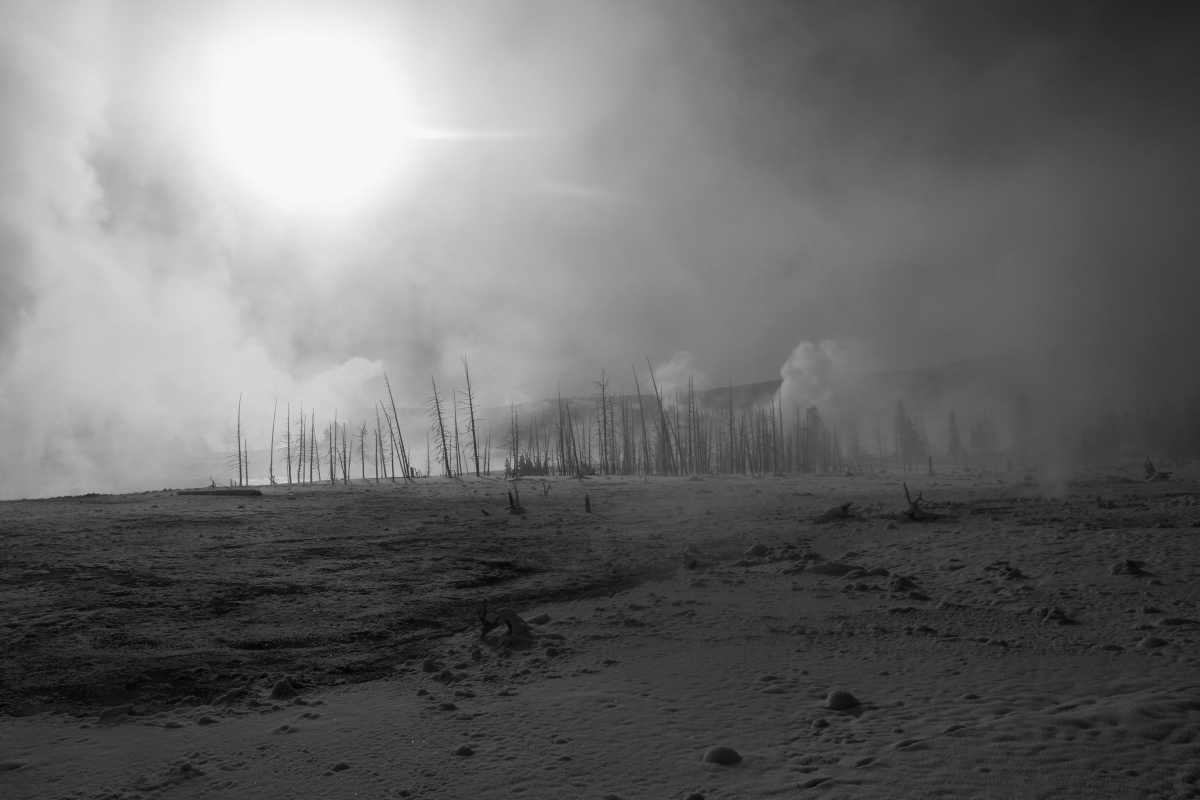
\includegraphics[width=0.4\textwidth]{TestImage.png}
    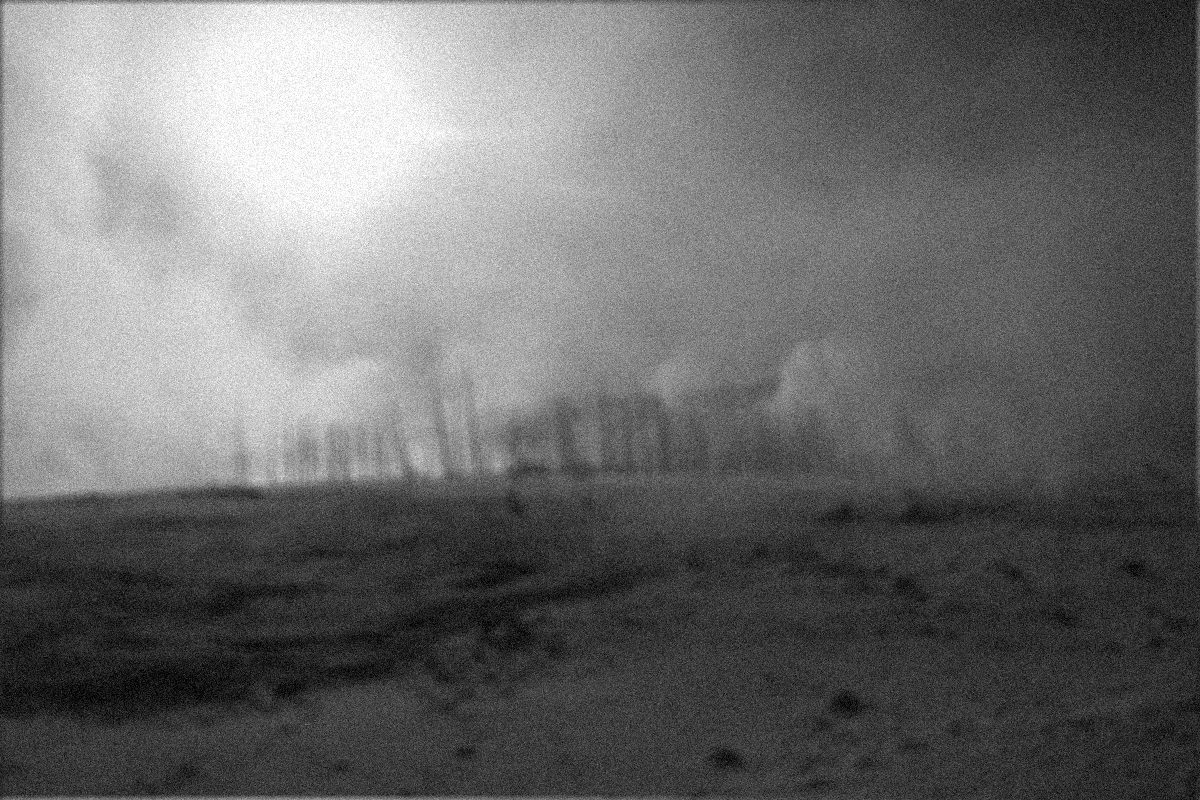
\includegraphics[width=0.4\textwidth]{testNoise_05.png}
\end{figure}

\solspace


\end{document}